\documentclass[8pt]{beamer}
%\setbeamertemplate{theorems}[numbered]

\usepackage{tikz}
\usepackage{xfrac}
\usepackage{mathtools}

\usetikzlibrary{shapes,shapes.geometric,shapes.multipart}
\usetheme{Boadilla}
\usefonttheme{structuresmallcapsserif}
\usecolortheme{rose}

\author{Gilad Hoch}
\date{25.3.2014}

\theoremstyle{plain}

\newtheorem{thm}{Theorem}
\newtheorem{dfn}[thm]{Definition}      
\newtheorem{corr}[thm]{Corollary}      
\newtheorem{lem}[thm]{Lemma}
\newtheorem{prop}[thm]{Proposition}
\newtheorem{clm}[thm]{Claim}           
\newtheorem{nota}[thm]{Notation}            
\newtheorem{property}[thm]{Property}
\newtheorem{algorithm}[thm]{Algorithm}            
\newtheorem{conjecture}[thm]{Conjecture}           

\DeclarePairedDelimiter\floor{\lfloor}{\rfloor}
\DeclarePairedDelimiter\ceil{\lceil}{\rceil}

\begin{document}
  \frame{
    \begin{center}
      \textsc{\Huge{Towards Polynomial Lower Bounds for Dynamic Problems}}
    \end{center}
%    \maketitle
%    \begin{enumerate}
%      \item presenting a few dynamic problems
%      \item defining the multiphase problem
%      \item conjecture 1. the multiphase conjecture
%      \item implications of the multiphase conecture
%      \item the $3SUM$ problem
%      \item ...
%    \end{enumerate}
  }

  \frame{
    \begin{itemize}
      \item \textbf{dynamic reachability:} maintain a data structure representing a directed graph which supports the following actions: 
	\begin{enumerate}
	  \item $insert(u,v)$ - insert an edge between $u$ and $v$
	  \item $delete(u,v)$ - delete the edge between $u$ and $v$
	  \item $reachability(u,v)$ - is there a directed path from $u$ to $v$?
	\end{enumerate}
      \item \textbf{dynamic shortest paths:} maintain a data structure representing an undirected graph which supports the following actions: 
	\begin{enumerate}
	  \item $insert(u,v)$ - insert an edge between $u$ and $v$
	  \item $delete(u,v)$ - delete the edge between $u$ and $v$
	  \item $length(u,v)$ - what is the length of the shortest path from $u$ to $v$?
	\end{enumerate}
      \item \textbf{subgraph connectivity:} preprocess undirected graphs to support the actions:
	\begin{enumerate}
	  \item $toggle(u)$ - turn node $u$ on/off
	  \item $connectivity(u,v)$ - is there a path between $u$ and $v$ that passes only in ``on'' nodes?
	\end{enumerate}
      \item \textbf{Langerman's problems:} maintain an array $A[1,\dots,n]$ of integers, under the following actions:
	\begin{enumerate}
	  \item $update(i,x)$ - $A[i]\leftarrow x$
	  \item $zeroSum$ - is there a $k$ such that $\sum_{i=1}^{k}{A[i]}=0$ ?
	\end{enumerate}
      \item \textbf{Pagh's problem:} preprocess a family of sets $X_1,X_2,\dots\subseteq[n]$ to support the following actions:
	\begin{enumerate}
	  \item $create(i,j)$ - create a new set $X_{new}\leftarrow{A_i\cap{A_j}}$
	  \item $query(i,z)$ - determine if $z\in{A_i}$
	\end{enumerate}
      \item \textbf{Erickson's problem:} preprocess an integers matrix $M$ to support:
	\begin{enumerate}
	  \item $incrementRow(M,i)$ - increment all values in row $i$
	  \item $incrementCol(M,i)$ - increment all values in column $i$
	  \item $max(M)$ - return the maximum value in the matrix
	\end{enumerate}
    \end{itemize}
  }
  
  \frame{
    \begin{center}
      \textsc{\huge{the multiphase problem}}
    \end{center}
    \setlength{\leftmargini}{75pt}
      \begin{enumerate}
	\item[\emph{phase   I}] pre-process an input of $k$ sets, $S_1,\dots,S_k\subset[n]$ in time $O(nk\cdot\tau)$ \linebreak(build a data structure for the next phases)
	\item[\emph{phase  II}] process yet another input of a set $T\subseteq[n]$ in time $O(n\cdot\tau)$ \linebreak(update the data structure from phase I)
	\item[\emph{phase III}] answer queries: given an index $i\in[k]$, determine if $S_i\cap{T}=\varnothing$
      \end{enumerate}


  }
  
  \frame{
    \begin{center}
      \textsc{\huge{the multiphase problem}}
    \end{center}
    \setlength{\leftmargini}{75pt}
    \begin{enumerate}
      \item[\emph{phase   I}] pre-process an input of $k$ sets, $S_1,\dots,S_k\subset[n]$ in time $O(nk\cdot\tau)$ \linebreak(build a data structure for the next phases)
      \item[\emph{phase  II}] process yet another input of a set $T\subseteq[n]$ in time $O(n\cdot\tau)$ \linebreak(update the data structure from phase I)
      \item[\emph{phase III}] answer queries: given an index $i\in[k]$, determine if $S_i\cap{T}=\varnothing$
    \end{enumerate}    
    
    \begin{conjecture}[1]
    $\exists$ constants $\gamma>1$, and $\delta>0$ \linebreak such that: $k=\Theta(n^\gamma)\Longrightarrow\tau=\Omega(n^\delta)$
    \end{conjecture}
  }
  
  \frame{
    \begin{center}
      \textsc{\huge{the multiphase problem}}
    \end{center}
    \setlength{\leftmargini}{75pt}
    \begin{enumerate}
      \item[\emph{phase   I}] pre-process an input of $k$ sets, $S_1,\dots,S_k\subset[n]$ in time $O(nk\cdot\tau)$ \linebreak(build a data structure for the next phases)
      \item[\emph{phase  II}] process yet another input of a set $T\subseteq[n]$ in time $O(n\cdot\tau)$ \linebreak(update the data structure from phase I)
      \item[\emph{phase III}] answer queries: given an index $i\in[k]$, determine if $S_i\cap{T}=\varnothing$
    \end{enumerate}    
    
    \begin{conjecture}[1]
    $\exists$ constants $\gamma>1$, and $\delta>0$ \linebreak such that: $k=\Theta(n^\gamma)\Longrightarrow\tau=\Omega(n^\delta)$
    \end{conjecture}
    
    \begin{thm}[2]
    if the multiphase problem is hard (in the sense of the conjecture) $\Longrightarrow$ for every problem we saw previously $\exists\epsilon>0$ such that the problem cannot be solved with $O(N^\epsilon)$ per operation and $O(N^{1+\epsilon})$ pre-processing time.
    \end{thm}
  }
  
  \frame{
    \begin{center}
      \textsc{\huge{the 3SUM problem}}
    \end{center}
    \setlength{\leftmargini}{30pt}
    \begin{enumerate}
      \item[\emph{input:}] a set $S$ of $n$ numbers
      \item[\emph{output:}] find distinct $x,y,z\in{S}$ such that $x+y=z$
    \end{enumerate}    
  }
  
  \frame{
    \begin{center}
      \textsc{\huge{the 3SUM problem}}
    \end{center}
    \setlength{\leftmargini}{30pt}
    \begin{enumerate}
      \item[\emph{input:}] a set $S$ of $n$ numbers
      \item[\emph{output:}] find distinct $x,y,z\in{S}$ such that $x+y=z$
    \end{enumerate}   
    
    \begin{thm}[3]
    Under the 3SUM conjecture, the multiphase problem with $k=\Theta(n^{2.5})$ requires $\tau\ge{n^{0.5-o(1)}}$ on the word RAM.
    \end{thm}
  }    
  
  \frame{
    \begin{center}
      \textsc{\huge{the 3SUM problem}}
    \end{center}
    \setlength{\leftmargini}{30pt}
    \begin{enumerate}
      \item[\emph{input:}] a set $S$ of $n$ numbers
      \item[\emph{output:}] find distinct $x,y,z\in{S}$ such that $x+y=z$
    \end{enumerate}   
    
    \begin{thm}[3]
    Under the 3SUM conjecture, the multiphase problem with $k=\Theta(n^{2.5})$ requires $\tau\ge{n^{0.5-o(1)}}$ on the word RAM.
    \end{thm}
    
    \begin{thm}[4]
    In a weighted graph with $m$ edges, finding a triangle of prescribed weight in $O(m^{1.5-\epsilon})$ time is 3SUM-hard.
    \end{thm}
    
    \begin{thm}[5]
    In a graph with $m$ edges, reporting $m$ triangles in $O(m^{\sfrac{4}{3}-\epsilon})$ time is 3SUM-hard.
    \end{thm}

  }    
  
  \frame{
    \begin{center}
      \textsc{\huge{the 3SUM problem}}
    \end{center}
    \setlength{\leftmargini}{30pt}
    \begin{enumerate}
      \item[\emph{input:}] a set $S$ of $n$ numbers
      \item[\emph{output:}] find distinct $x,y,z\in{S}$ such that $x+y=z$
    \end{enumerate}   
    
    \begin{conjecture}[6: 3SUM-HARDNESS]
    in the word RAM model with words of $O(\log(n))$ bits, any algorithm requires $n^{2-o(1)}$ time in expectation to determine whether a set $S\subset\{-n^3,\dots,n^3\}$ of $|S|=n$ integers contains a triple of distinct $x,y,z\in{S}$ with $x+y=z$.
    \end{conjecture}
  }

  \frame{
    \begin{center}
      \textsc{\huge{Convolution 3SUM}}
    \end{center}
    \setlength{\leftmargini}{30pt}
    \begin{enumerate}
      \item[\emph{input:}] an Array $A[1..n]$ of $n$ integers
      \item[\emph{output:}] find 2 indexes $i\ne{j}$ such that $A[i]+A[j]=A[i+j]$
    \end{enumerate}   
  }
  
  \frame{
    \begin{center}
      \textsc{\huge{Convolution 3SUM}}
    \end{center}
    \setlength{\leftmargini}{30pt}
    \begin{enumerate}
      \item[\emph{input:}] an Array $A[1..n]$ of $n$ integers
      \item[\emph{output:}] find 2 indexes $i\ne{j}$ such that $A[i]+A[j]=A[i+j]$
    \end{enumerate} 
    \begin{thm}[10]
      If 3SUM requires $\Omega(\sfrac{n^2}{f(n)})$ expected time, convolution-3SUM requires $\Omega(\sfrac{n^2}{f^2(n\cdot{f(n)})})$ expected time.
    \end{thm}
  }  
  
  \frame{
    \begin{center}
      \textsc{\huge{Convolution 3SUM}}
    \end{center}
    \setlength{\leftmargini}{30pt}
    \begin{enumerate}
      \item[\emph{input:}] an Array $A[1..n]$ of $n$ integers
      \item[\emph{output:}] find 2 indexes $i\ne{j}$ such that $A[i]+A[j]=A[i+j]$
    \end{enumerate} 
    \begin{thm}[10]
      If 3SUM requires $\Omega(\sfrac{n^2}{f(n)})$ expected time, convolution-3SUM requires $\Omega(\sfrac{n^2}{f^2(n\cdot{f(n)})})$ expected time.
    \end{thm}
    \begin{center}
      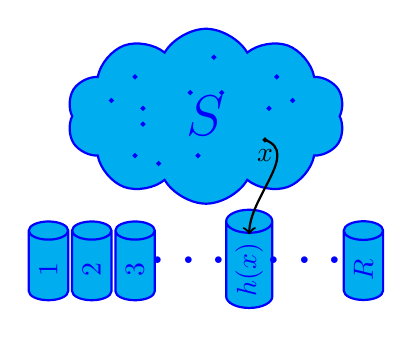
\begin{tikzpicture}
      
      \node [cloud, thick, blue, fill=cyan, draw,cloud puffs=10,cloud puff arc=120, aspect=2, inner ysep=1em] at (0,0) {\huge{$S$}};
%       \draw [thick, blue, fill=cyan] (0.6,1)   to [out=0,in=108] 
% 				      (1.2,0.6) to [out=288,in=36] 
% 				      (1.4,0)   to [out=216,in=324] 
% 				      (0.3,0)   to [out=144,in=288] 
% 				      (0,0.6)   to [out=108,in=180]
% 				      (0.6,1);
%       \node [below, blue] at (0.6,0.75) {\huge{$S$}};
      \draw[fill, blue] (-1.2,0.2) circle [radius=0.025];
      \draw[fill, blue] (0.9,0.5) circle [radius=0.025];
      \draw[fill, blue] (0.8,0.1) circle [radius=0.025];
      \draw[fill, blue] (0.1,0.75) circle [radius=0.025];
      \draw[fill, blue] (0.2,0.3) circle [radius=0.025];
      \draw[fill, blue] (-0.9,0.5) circle [radius=0.025];
      \draw[fill, blue] (-0.8,0.1) circle [radius=0.025];
      \draw[fill, blue] (-0.6,-0.6) circle [radius=0.025];
      \draw[fill, blue] (-0.9,-0.5) circle [radius=0.025];
      \draw[fill, blue] (-0.8,-0.1) circle [radius=0.025];
      \draw[fill, blue] (-0.1,-0.5) circle [radius=0.025];
      \draw[fill, blue] (-0.2,0.3) circle [radius=0.025];
      \draw[fill, blue] (1.1,0.2) circle [radius=0.025];
      
      \node[cylinder,thick, blue, fill=cyan, draw,rotate=90,shape aspect=.5,minimum height=1cm,minimum width=0.5cm] at (-2,-1.95) {$1$};
      \node[cylinder,thick, blue, fill=cyan, draw,rotate=90,shape aspect=.5,minimum height=1cm,minimum width=0.5cm] at (-1.45,-1.95) {$2$};
      \node[cylinder,thick, blue, fill=cyan, draw,rotate=90,shape aspect=.5,minimum height=1cm,minimum width=0.5cm] at (-0.9,-1.95) {$3$};
      \node[cylinder,thick, blue, fill=cyan, draw,rotate=90,shape aspect=.5,minimum height=1cm,minimum width=0.5cm] at (0.55,-1.95) {$h(x)$};
      \node[cylinder,thick, blue, fill=cyan, draw,rotate=90,shape aspect=.5,minimum height=1cm,minimum width=0.5cm] at (2,-1.95) {$R$};
      
      \node[above, blue] at (-0.15,-2) {\Huge{$\dots$}};
      \node[above, blue] at (1.325,-2) {\Huge{$\dots$}};
      
      \draw[fill] (0.75,-0.3) circle [radius=0.025];
      \node[below] at (0.75,-0.3) {$x$};
      \draw[->,thick] (0.75,-0.3) to [out=340,in=90] (0.55,-1.5);
      \end{tikzpicture}
    \end{center}
  }  
  
  \frame{
    \begin{center}
      \textsc{\huge{Convolution 3SUM}}
    \end{center}
%     \setlength{\leftmargini}{30pt}
%     \begin{enumerate}
%       \item[\emph{input:}] an Array $SA[1..n]$ of $n$ integers
%       \item[\emph{output:}] find 2 indexes $i\ne{j}$ such that $A[i]+A[j]=A[i+j]$
%     \end{enumerate} 
%     \begin{thm}[10]
%       If 3SUM requires $\Omega(\sfrac{n^2}{f(n)})$ expected time, convolution-3SUM requires $\Omega(\sfrac{n^2}{f^2(n\cdot{f(n)})})$ expected time.
%     \end{thm}
    \begin{center}
      \begin{tikzpicture}
      \node[cylinder,thick, blue, fill=cyan, draw,rotate=90,shape aspect=1,minimum height=4cm,minimum width=1cm] at (-4,0) {}; \node[below, blue] at (-4,-2) {$1$};
      \node[cylinder,thick, blue, fill=cyan, draw,rotate=90,shape aspect=1,minimum height=4cm,minimum width=1cm] at (-2.9,0) {}; \node[below, blue] at (-2.9,-2) {$2$};
      \node[cylinder,thick, blue, fill=cyan, draw,rotate=90,shape aspect=1,minimum height=4cm,minimum width=1cm] at (-1.8,0) {}; \node[below, blue] at (-1.8,-2) {$3$};
      \node[cylinder,thick, blue, fill=cyan, draw,rotate=90,shape aspect=1,minimum height=4cm,minimum width=1cm] at (1.1,0) {}; \node[below, blue] at (1.1,-2) {$t$};
      \node[cylinder,thick, blue, fill=cyan, draw,rotate=90,shape aspect=1,minimum height=4cm,minimum width=1cm] at (4,0) {}; \node[below, blue] at (4,-2) {$R$};
      
      \node[above, blue] at (-0.3,0) {\Huge{$\dots$}};
      \node[above, blue] at (2.65,0) {\Huge{$\dots$}};
      
      \node[rectangle split, blue, fill=lime, draw,rectangle split parts=9] at (1.1,0) {
	$\sfrac{3n}{R}$ 
	\nodepart{two} \dots 
	\nodepart{three} $k$    
	\nodepart{four} \dots  
	\nodepart{five} $j$  
	\nodepart{six} \dots  
	\nodepart{seven} $i$   
	\nodepart{eight} \dots 
	\nodepart{nine} 1
      };
      
      \node[rectangle split, blue, fill=cyan, draw,rectangle split horizontal,rectangle split parts=5,text height=0.4cm,text width=1.6cm,rectangle split empty part width=1.5cm,align=center] at (0,-3.2) {
      \nodepart{one} $1$
      \nodepart{two} \Huge{\dots}
      \nodepart{four} \Huge{\dots}
      \nodepart{five} $O(R)$
      };
      
      \node[rectangle split, blue, fill=lime, draw,rectangle split horizontal,rectangle split parts=5,text height=0.2cm,text width=0.1cm,align=center] at (0,-3.2) {};
      \draw[->,thick] (0.95,-0.75) to [out=180,in=90] (-0.675,-3.2);
      \draw[->,thick] (1.25,-0.1) to [out=0,in=60] (2,-2) to [out=240,in=90] (0,-3.2);
      \draw[->,thick] (1.25,0.6) to [out=0,in=60] (2.1,-2.2) to [out=240,in=90] (0.325,-3.2);
      
      \node[above//below] at (0.666,-3.2) {\tiny{$...$}};
      \node[above//below] at (-0.366,-3.2) {\footnotesize{$M$}};
      \end{tikzpicture}
    \end{center}
  }

  \frame{
    \begin{center}
      \textsc{\huge{Hardness of Reporting Triangles}}
    \end{center}
    \begin{lem}[11]
      Assume Convolution-3SUM requires $\Omega(\sfrac{n^2}{f(n)})$ expected time, and let $R$ be:
      $$\omega(\sqrt{n\cdot{f(n)}})<R<o(\sfrac{n}{f(n)})$$.
      Then, $\Omega(\sfrac{n^2}{f(n)})$ expected time is needed to report $O(\sfrac{n^2}{R})$ triangles in a tripartite graph where:
      \begin{itemize}
       \item the three parts are $A,B,C$, of sizes $|A|=|B|=R\sqrt{n}$ and $|C|=n$;
       \item each vertex in $A\cup{B}$ has $O(\sfrac{n}{R})$ neighbors in $C$;
       \item there are $O(nR)$ edges in $A\times{B}$.
      \end{itemize}

    \end{lem}
  }  
  
  \frame{
    \begin{center}
      \textsc{\huge{Hardness of Reporting Triangles}}
    \end{center}
%     \begin{lem}[11]
%       Assume Convolution-3SUM requires $\Omega(\sfrac{n^2}{f(n)})$ expected time, and let $R$ be:
%       $$\omega(\sqrt{n\cdot{f(n)}})<R<o(\sfrac{n}{f(n)})$$.
%       Then, $\Omega(\sfrac{n^2}{f(n)})$ expected time is needed to report $O(\sfrac{n^2}{R})$ triangles in a tripartite graph where:
%       \begin{itemize}
%        \item the three parts are $A,B,C$, of sizes $|A|=|B|=R\sqrt{n}$ and $|C|=n$;
%        \item each vertex in $A\cup{B}$ has $O(\sfrac{n}{R})$ neighbors in $C$;
%        \item there are $O(nR)$ edges in $A\times{B}$.
%       \end{itemize}
%     \end{lem}
    \begin{center}
      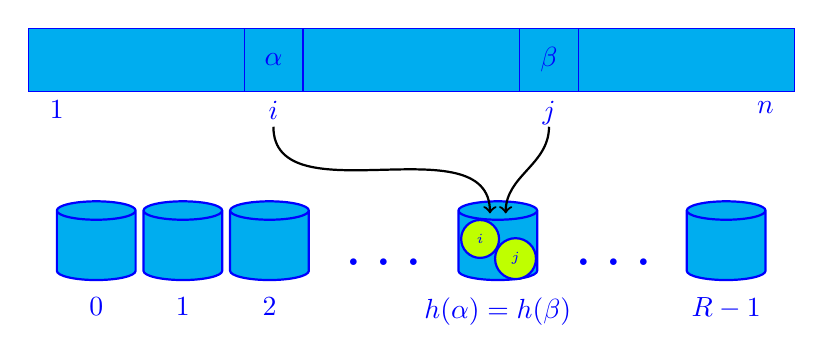
\begin{tikzpicture}
       \node[rectangle split, blue, fill=cyan, draw,rectangle split horizontal,rectangle split parts=5,text height=0.5cm,align=center] at (0,0.4) {
	\nodepart[text width=2.5cm]{one} 
	\nodepart[text width=0.5cm]{two} $\alpha$
	\nodepart[text width=2.5cm]{three} 
	\nodepart[text width=0.5cm]{four} $\beta$
	\nodepart[text width=2.5cm]{five} 
       };
       \node[below, blue] at (-4.5,0) {$1$};
       \node[below, blue] at (-1.75,0) {$i$};
       \node[below, blue] at (1.75,0) {$j$};
       \node[below, blue] at (4.5,0) {$n$};
       
       \node[cylinder,thick, blue, fill=cyan, draw,rotate=90,shape aspect=1,minimum height=1cm,minimum width=1cm] at (-4,-2) {}; \node[below, blue] at (-4,-2.5) {$0$};
       \node[cylinder,thick, blue, fill=cyan, draw,rotate=90,shape aspect=1,minimum height=1cm,minimum width=1cm] at (-2.9,-2) {}; \node[below, blue] at (-2.9,-2.5) {$1$};
       \node[cylinder,thick, blue, fill=cyan, draw,rotate=90,shape aspect=1,minimum height=1cm,minimum width=1cm] at (-1.8,-2) {}; \node[below, blue] at (-1.8,-2.5) {$2$};
       \node[cylinder,thick, blue, fill=cyan, draw,rotate=90,shape aspect=1,minimum height=1cm,minimum width=1cm] at (1.1,-2) {}; \node[below, blue] at (1.1,-2.5) {$h(\alpha)=h(\beta)$};
       \node[cylinder,thick, blue, fill=cyan, draw,rotate=90,shape aspect=1,minimum height=1cm,minimum width=1cm] at (4,-2) {}; \node[below, blue] at (4,-2.5) {$R-1$};
       \node[below, blue] at (2.65,-2) {\Huge{$\dots$}};
       \node[below, blue] at (-0.275,-2) {\Huge{$\dots$}};
       
       \draw[->,thick] (-1.75,-0.45) to [out=270,in=90] (1,-1.55);
       \draw[->,thick] (1.75,-0.45) to [out=270,in=90] (1.2,-1.55);
       
       \node[circle, thick, blue, fill=lime, draw] at (0.875,-1.875) {\tiny{$i$}};
       \node[circle, thick, blue, fill=lime, draw] at (1.325,-2.125) {\tiny{$j$}};
      \end{tikzpicture}
    \end{center}
  }
  
  \frame{
    \begin{center}
      \textsc{\huge{Hardness of Reporting Triangles}}
    \end{center}
    \begin{center}
      \begin{tikzpicture}
       \node[rectangle split, blue, fill=cyan, draw,rectangle split horizontal,rectangle split parts=3,text height=0.5cm,align=center] at (0,0.4) {
	\nodepart[text width=5cm]{one} 
	\nodepart[text width=0.5cm]{two} $\alpha$
	\nodepart[text width=3.5cm]{three} 
       };
       \node[below, blue] at (-4.5,0) {$1$};
       \node[below, blue] at (0.75,0) {$i$};
       \node[below, blue] at (4.5,0) {$n$};
       \draw[->,thick] (0.75,-0.45) to [out=270,in=90] (1,-1);
       \node[below, blue] at (1,-1) {$x\leftarrow{h(\alpha)}$};      
       
       \node[cylinder,thick, blue, fill=cyan, draw,rotate=90,shape aspect=.5,minimum height=1.25cm,minimum width=0.5cm] at (-4.5,-2.5) {$0$};
       \node[cylinder,thick, blue, fill=cyan, draw,rotate=90,shape aspect=.5,minimum height=1.25cm,minimum width=0.5cm] at (-3.95,-2.5) {$1$};
       \node[above//below,blue] at (-3.375,-2.5) {\large{$\dots$}};
       \node[cylinder,thick, blue, fill=cyan, draw,rotate=90,shape aspect=.5,minimum height=1.25cm,minimum width=0.5cm] at (-2.85,-2.5) {$y$};
       \node[above//below,blue] at (-2.275,-2.5) {\large{$\dots$}};
       \node[cylinder,thick, blue, fill=cyan, draw,rotate=90,shape aspect=.5,minimum height=1.25cm,minimum width=0.5cm] at (-1.75,-2.5) {$x+y$};
       \node[above//below,blue] at (-1.175,-2.5) {\large{$\dots$}};
       \node[cylinder,thick, blue, fill=cyan, draw,rotate=90,shape aspect=.5,minimum height=1.25cm,minimum width=0.5cm] at (-0.65,-2.5) {$R-1$};
       
       \node[below, blue] at (1.25,-2) {$\{j_1,\dots,j_{\sfrac{cn}{R}}\}$};    %\leftarrow{B(x+y)}
       \draw[->,thick] (-1.75,-1.7) to [out=90,in=120] (-0.5,-1.25) to [out=300,in=180] (0.2,-1.8) to [out=0,in=105] (1,-2);
       
       \node[below, blue] at (2.1,-3) {$T\leftarrow\{j_1-i,\dots,j_{\sfrac{cn}{R}}-i\}$};
       
       \node[below, blue] at (1.5,-4) {$\{{j'}_1,\dots,{j'}_{\sfrac{c'n}{R}}\}$};
       \draw[->,thick] (-2.85,-3.1) to [out=270,in=180] (-1.25,-4) to [out=0,in=120] (1,-4);
       
       \node[below, blue] at (2.1,-5) {$\{{j'}_1,\dots,{j'}_{\sfrac{c'n}{R}}\}\cap{T}\ne\varnothing$};
      \end{tikzpicture}
    \end{center}
  }
  
  \frame{
    \begin{center}
      \textsc{\huge{Hardness of Reporting Triangles}}
    \end{center}
    \begin{center}
      \begin{tikzpicture}
       \node[rectangle split, blue, fill=cyan, draw,rectangle split horizontal,rectangle split parts=5,text height=0.5cm,align=center] at (0,0.4) {
	\nodepart[text width=0.5cm]{one} 
	\nodepart[text width=2cm]{two} 
	\nodepart[text width=0.5cm]{three} 
	\nodepart[text width=5.1cm]{four} 
	\nodepart[text width=0.5cm]{five} 
       };
       \node[above//below, blue] at (-4.5,0.35) {$1$};
       \node[above//below, blue] at (-1.55,0.35) {$i$};
       \node[above//below, blue] at (4.5,0.35) {$n$};  
       
       
       \node[above//below, blue] at (-1.55,1) {$i_1=i (mod \sqrt{n}),i_2=\floor{\frac{i}{\sqrt{n}}}$};
       
       \node[cylinder,thick, blue, fill=cyan, draw,rotate=90,shape aspect=.5,minimum height=1.25cm,minimum width=0.5cm] at (-4.5,-2.5) {$0$};
       \node[cylinder,thick, blue, fill=cyan, draw,rotate=90,shape aspect=.5,minimum height=1.25cm,minimum width=0.5cm] at (-3.95,-2.5) {$1$};
       \node[above//below,blue] at (-3.375,-2.5) {\large{$\dots$}};
       \node[cylinder,thick, blue, fill=cyan, draw,rotate=90,shape aspect=.5,minimum height=1.25cm,minimum width=0.5cm] at (-2.85,-2.5) {$x_2$};
       \node[above//below,blue] at (-2.275,-2.5) {\large{$\dots$}};
       \node[cylinder,thick, blue, fill=cyan, draw,rotate=90,shape aspect=.5,minimum height=1.25cm,minimum width=0.5cm] at (-1.75,-2.5) {$x_1$};
       \node[above//below,blue] at (-1.175,-2.5) {\large{$\dots$}};
       \node[cylinder,thick, blue, fill=cyan, draw,rotate=90,shape aspect=.5,minimum height=1.25cm,minimum width=0.5cm] at (-0.65,-2.5) {$R-1$};
       
       \node [cloud, thick, blue, fill=cyan, draw,cloud puffs=10,cloud puff arc=120, aspect=2, inner ysep=1em] at (3.5,-1.5) {\huge{$A$}};
       \node [cloud, thick, blue, fill=cyan, draw,cloud puffs=10,cloud puff arc=120, aspect=2, inner ysep=1em] at (0.25,-5.5) {\huge{$B$}};
       \node [cloud, thick, blue, fill=cyan, draw,cloud puffs=10,cloud puff arc=120, aspect=2, inner ysep=1em] at (3.75,-4.5) {\huge{$C$}};
       
       
       \draw[-,very thick, red] (3.3,-4.5) to [out=90,in=270](2.85,-1.75);
       
       \foreach [count=\i] \p in {(2.9,-4.3),(3.3,-4.5),(3.7,-3.9),(4.1,-4.1)}{
         \draw[-] \p  to [out=90,in=270](2.85,-1.75);
         \draw[fill, blue] \p circle [radius=0.04];
         \draw[fill, lime] \p circle [radius=0.025];
         \node[below, blue] at \p {\tiny{${j'_\i}$}};
       }
       
       \node[rectangle,cyan,fill=cyan, draw, minimum height=0.4cm,minimum width=0.4cm] at (3.3,-4.8) {}; %hide j'_2
       
       \foreach [count=\i] \p in {(4.3,-4.85),(4.7,-4.75),(3.9,-5.15)}{
         \draw[-] \p  to [out=270,in=0] (1.175,-5.5);
         \draw[fill, blue] \p circle [radius=0.04];
         \draw[fill, lime] \p circle [radius=0.025];
         \node[above, blue] at \p {\tiny{${k'_\i}$}};
       }
       
       \draw[-,very thick, red] (2.85,-1.5) to [out=180,in=0] (0.925,-5.5);
       \draw[-] (2.85,-1.5) to [out=180,in=0] (0.925,-5.5);
       
       \draw[-,very thick, red] (3.3,-4.5) to [out=210,in=0] (1.175,-5.5);
       \draw[-] (3.3,-4.5) to [out=210,in=0] (1.175,-5.5);
       \draw[fill, blue] (3.3,-4.5) circle [radius=0.04];
       \draw[fill, lime] (3.3,-4.5) circle [radius=0.025];
       \node[below, blue] at (3.325,-4.55) {\tiny{$j'_2=k'_4$}};
      
       \node[circle, thick, blue, fill=lime, draw] at (2.85,-1.5) {\footnotesize{$(x_1,i_1)$}};
       \draw[-,thick] (-1.5,0) to [out=270,in=90] (-1.5,-0.1) to [out=270,in=90] (-4.1,-0.55) to [out=270,in=180] (-3.8,-0.75);   
       \draw[->,thick] (-1.75,-1.75) to [out=90,in=270](-4.1,-1) to [out=90,in=180] (-3.8,-0.75); 
       \node[above//below, blue] at (-0.9,-0.75) {$\{j_1-i_1,\dots,j_{\sfrac{cn}{R}}-i_1\}=\{{j'}_1,{j'}_2,{j'}_3,{j'}_4,\dots\}$};
       \draw[->,thick] (2,-0.75) to [out=0,in=90] (2.85,-1.25); 
       
       \node[circle, thick, blue, fill=lime, draw] at (0.925,-5.5) {\footnotesize{$(x_2,i_2)$}};
       \draw[->,thick] (-1.6,0) to [out=270,in=0] (-3.6,-0.05) to [out=180,in=180] (-4,-4);  
       \draw[-,thick] (-2.85,-3.1) to [out=270,in=0](-3.25,-3.625) to [out=180,in=90] (-4.5,-3.5) to [out=270,in=180] (-4,-4);  
       \node[above, blue] at (-1.65,-4.275) {$\{k_1+i_2\cdot{\sqrt{n}},\dots,k_{\sfrac{c'n}{R}}+i_2\cdot{\sqrt{n}}\}=$};
       \node[below, blue] at (-2.55,-4.2) {$\{{k'}_1,{k'}_2,{k'}_3,{k'}_4,\dots\}$};
       \draw[->,thick] (-1.1,-4.45) to [out=0,in=90] (0.925,-5.25); 

      \end{tikzpicture}
    \end{center}
  }
  
\end{document}
